\documentclass{beamer}

\usetheme{default}

\title{Wpływ współczesnego świata na język japoński}
\author{Kamil Karaś}
\date{\today}

\usepackage{tikz}
\usepackage[T1]{fontenc}

\begin{document}

    \begin{frame}
        \titlepage
    \end{frame}

    \begin{frame}
        \tableofcontents
    \end{frame}

    \section{Historia chińskich znaków}
    \section{Zapomniana Man'yougana}
    \section{Obecna katakana oraz hiragana}
    \section{Bibliografia}

    
\begin{frame}
    \begin{block}{Historia chińskich znaków}
        Znaki chińskie \#\# (kanji) przypłynęły w postaci świętych ksiąg buddyjskich, kronik itp. w okolicach V wieku. Wraz z ich popularyzacją znajomość tych znaków świadczyła o wysokim wyedukowaniu. Mnisi japońscy studiowali księgi i zaczęli używać znaków chińskich w języku japońskim w celu opisywania nowych terminów. Na przykład sformułowań wywodzących się z buddyzmu. 
    \end{block}
    

\end{frame}

\begin{frame}
    \begin{tikzpicture}[remember picture, overlay]
        \node[] at (current page.center){
            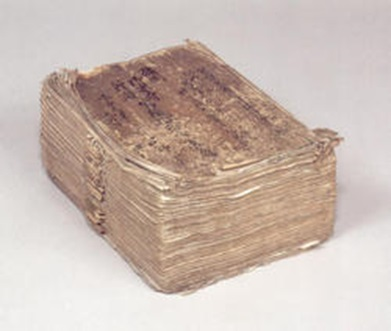
\includegraphics[width=1\textwidth]{images/image1.jpg}
        };
    \end{tikzpicture}
\end{frame}
    
\begin{frame}
    \begin{block}{Zapomniana Man'yougana}
        W VII wieku na podstawie chińskich znaków stworzono uproszczony alfabet zwany \#\#\#\# (man-you-ga-na). Był to pierwszy alfabet stworzony do reprezentowania japońskiego języka z myślą o fonetyce. Znaczenia znaków w języku chińskim były całkowicie pomijane i używane jedynie, aby odzwierciedlić wymowę danego słowa japońskiego na piśmie. Przykładowo, aby stworzyć słowo naka znaczące środek, wewnątrz rozbijano słowo na mora czyli sylaby. W słowie naka znajdują się dwie sylaby odpowiednio: na oraz ka. Sylabę na można zaprezentować używając znaku \#, natomiast sylabę ka znaku \#. W wyniku powstaje nam \#\#.
    \end{block}
    
\end{frame} 

\begin{frame}
    \begin{tikzpicture}[remember picture, overlay]
        \node[] at (current page.center){
            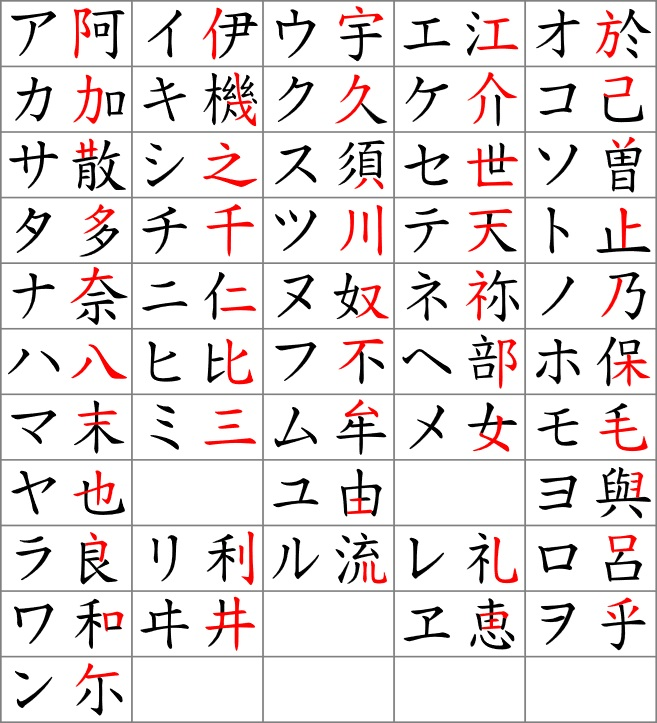
\includegraphics[width=1\textwidth]{images/image2.jpg}
        };
    \end{tikzpicture}
\end{frame}

\begin{frame}
    \begin{block}{Obecna katakana oraz hiragana}
        W obecnym stuleciu pojawiały się pomysły mówiące o całkowitym zniesieniu znaków kanji na rzecz tylko tych dwóch prostszych alfabetów używanych do dziś, jednak plan nie wszedł w życie. Składa się na tą decyzję kilka powodów, jednak jednymi z najważniejszych są: tradycja, przyzwyczajenie, ilość pieniędzy jaką musiano by zainwestować w zmiany różnych elementów infrastruktury, wydruk nowych książek, zmianę systemu pisania, itd. 
    \end{block}
        

\end{frame}

\begin{frame}
    \begin{tikzpicture}[remember picture, overlay]
        \node[] at (current page.center){
            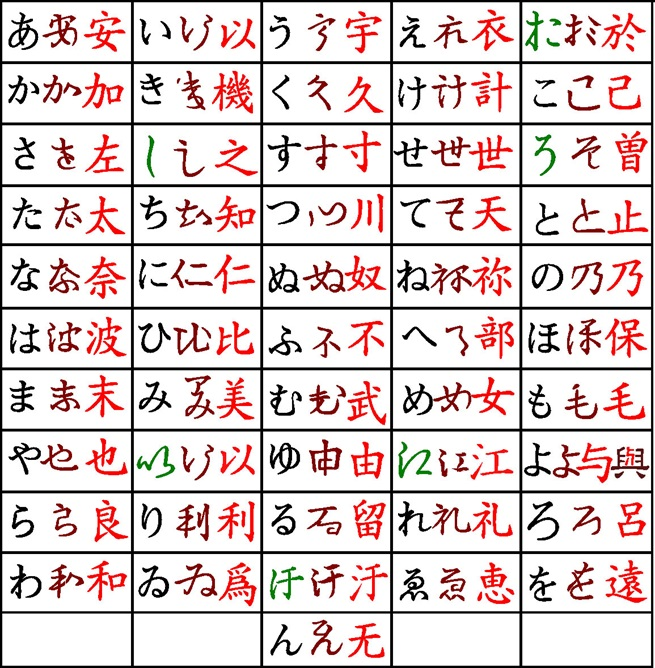
\includegraphics[width=1\textwidth]{images/image3.jpg}
        };
    \end{tikzpicture}
\end{frame}

\end{document}
